\documentclass{standalone}

\usepackage{tikz}
\usepackage[T1]{fontenc}
\usepackage[tt=false, type1=true]{libertine}
\usepackage[varqu]{zi4}
\usepackage[libertine]{newtxmath}

\usetikzlibrary{shapes, positioning, calc}

\begin{document}

{\scriptsize
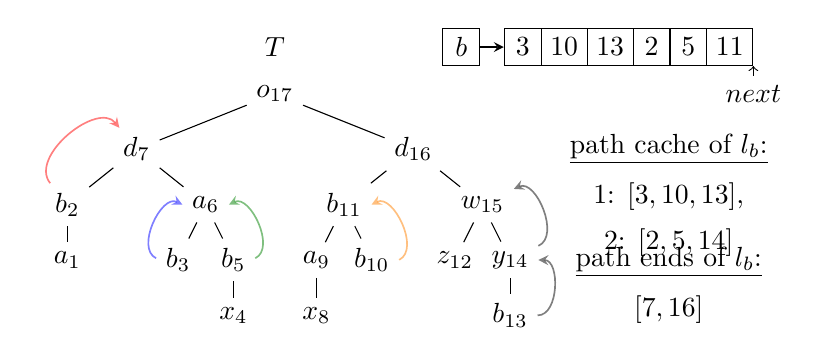
\begin{tikzpicture}[
    level distance=2em,
    level 1/.style={sibling distance=10em},
    level 2/.style={sibling distance=5em},
    level 3/.style={sibling distance=2em}]
  \newcommand\listspacing{0.1}
  \newcommand\listpartspacing{0.3}
  \newcommand\arraypartspacing{0.015} % 0.03 for thick
  \newcommand\listdir{right}
  \newcommand\lbldir{below}

  \tikzset{ptr/.style={semithick, ->, >=stealth}}
  \tikzset{shincolorptr/.style={ptr, opacity=0.5}}
  \tikzset{shincolorrptr/.style={shincolorptr, red}}
  \tikzset{shincolorbptr/.style={shincolorptr, blue}}
  \tikzset{shincolorgptr/.style={shincolorptr, black!50!green}}
  \tikzset{shincoloroptr/.style={shincolorptr, orange}}
  \tikzset{shincolorgrptr/.style={shincolorptr, black}}
  \tikzset{ilentry/.style={draw, minimum width=0.4675cm, minimum height=0.4675cm}}

  % document
  \node at (0, 0) (t-root) {$o_{17}$}
  child {
    node (d7) {$d_7$}
    child {
      node (b2) {$b_2$}
      child { node (a1) {$a_1$} }
    }
    child {
      node (a6) {$a_6$}
      child { node (b3) {$b_3$} }
      child {
        node (b5) {$b_5$}
        child { node (x4) {$x_4$} }
      }
    }
  }
  child {
    node (d16) {$d_{16}$}
    child {
      node (b11) {$b_{11}$}
      child {
        node (a9) {$a_9$}
        child { node (x8) {$x_8$} }
      }
      child { node (b10) {$b_{10}$} }
    }
    child {
      node (w15) {$w_{15}$}
      child { node (z12) {$z_{12}$} }
      child {
        node (y14) {$y_{14}$}
        child { node (b13) {$b_{13}$} }
      }
    }
  };
  \node[above=0.125 of t-root] (t) {$T$};

  % inverted list
  \node[ilentry, \listdir=1.875 of t] (il) {$b$};
  \node[ilentry, \listdir=\listpartspacing of il] (il-1) {$3$};
  \foreach \val/\id [count=\previd from 1] in {10/2, 13/3, 2/4, 5/5, 11/6}{
    \node[ilentry, \listdir=-\arraypartspacing of il-\previd] (il-\id) {$\val$};
  }
  \draw[ptr] (il) -- (il-1);
  \draw[<-] (il-6.south east) -- ++(0, -0.125) node[below] {$next$};

  % path cache
  \node[\listdir=1.5 of d16] (pc) {\underline{path cache of $l_b$:}};
  \node[\lbldir=-\arraypartspacing of pc] (pc-b1) {$1$: $\left[3, 10, 13\right]$,};
  \node[\lbldir=-\arraypartspacing of pc-b1] (pc-b2) {$2$: $\left[2, 5, 14\right]$};

  % path ends of list l_b
  \node[\lbldir=8*\listspacing of pc] (pe) {\underline{path ends of $l_b$:}};
  \node[\lbldir=-\arraypartspacing of pe] {$\left[7, 16\right]$};

  % next of list l_b
  %\node[\lbldir=\listspacing of pe] (pc) {next pos. in $l_b$: $6$};

  \draw[shincolorrptr] (b2) to[bend left=90] (d7);
  \draw[shincolorbptr] (b3) to[bend left=90] (a6.west);
  \draw[shincolorgptr] (b5) to[bend right=90] (a6.east);
  \draw[shincoloroptr] (b10) to[bend right=90] (b11.east);
  \draw[shincolorgrptr] (b13) to[bend right=90] (y14);
  \draw[shincolorgrptr] (y14) to[bend right=90] (w15);
\end{tikzpicture}}

\end{document}
